% Generated by Sphinx.
\def\sphinxdocclass{report}
\documentclass[letterpaper,10pt,english]{sphinxmanual}
\usepackage[utf8]{inputenc}
\DeclareUnicodeCharacter{00A0}{\nobreakspace}
\usepackage{cmap}
\usepackage[T1]{fontenc}
\usepackage{babel}
\usepackage{times}
\usepackage[Bjarne]{fncychap}
\usepackage{longtable}
\usepackage{sphinx}
\usepackage{multirow}


\title{code\_web\_portal Documentation}
\date{January 26, 2015}
\release{1.0.0}
\author{Oleksandr Zastupailo, Tatiana Vert}
\newcommand{\sphinxlogo}{}
\renewcommand{\releasename}{Release}
\makeindex

\makeatletter
\def\PYG@reset{\let\PYG@it=\relax \let\PYG@bf=\relax%
    \let\PYG@ul=\relax \let\PYG@tc=\relax%
    \let\PYG@bc=\relax \let\PYG@ff=\relax}
\def\PYG@tok#1{\csname PYG@tok@#1\endcsname}
\def\PYG@toks#1+{\ifx\relax#1\empty\else%
    \PYG@tok{#1}\expandafter\PYG@toks\fi}
\def\PYG@do#1{\PYG@bc{\PYG@tc{\PYG@ul{%
    \PYG@it{\PYG@bf{\PYG@ff{#1}}}}}}}
\def\PYG#1#2{\PYG@reset\PYG@toks#1+\relax+\PYG@do{#2}}

\expandafter\def\csname PYG@tok@gd\endcsname{\def\PYG@tc##1{\textcolor[rgb]{0.63,0.00,0.00}{##1}}}
\expandafter\def\csname PYG@tok@gu\endcsname{\let\PYG@bf=\textbf\def\PYG@tc##1{\textcolor[rgb]{0.50,0.00,0.50}{##1}}}
\expandafter\def\csname PYG@tok@gt\endcsname{\def\PYG@tc##1{\textcolor[rgb]{0.00,0.27,0.87}{##1}}}
\expandafter\def\csname PYG@tok@gs\endcsname{\let\PYG@bf=\textbf}
\expandafter\def\csname PYG@tok@gr\endcsname{\def\PYG@tc##1{\textcolor[rgb]{1.00,0.00,0.00}{##1}}}
\expandafter\def\csname PYG@tok@cm\endcsname{\let\PYG@it=\textit\def\PYG@tc##1{\textcolor[rgb]{0.25,0.50,0.56}{##1}}}
\expandafter\def\csname PYG@tok@vg\endcsname{\def\PYG@tc##1{\textcolor[rgb]{0.73,0.38,0.84}{##1}}}
\expandafter\def\csname PYG@tok@m\endcsname{\def\PYG@tc##1{\textcolor[rgb]{0.13,0.50,0.31}{##1}}}
\expandafter\def\csname PYG@tok@mh\endcsname{\def\PYG@tc##1{\textcolor[rgb]{0.13,0.50,0.31}{##1}}}
\expandafter\def\csname PYG@tok@cs\endcsname{\def\PYG@tc##1{\textcolor[rgb]{0.25,0.50,0.56}{##1}}\def\PYG@bc##1{\setlength{\fboxsep}{0pt}\colorbox[rgb]{1.00,0.94,0.94}{\strut ##1}}}
\expandafter\def\csname PYG@tok@ge\endcsname{\let\PYG@it=\textit}
\expandafter\def\csname PYG@tok@vc\endcsname{\def\PYG@tc##1{\textcolor[rgb]{0.73,0.38,0.84}{##1}}}
\expandafter\def\csname PYG@tok@il\endcsname{\def\PYG@tc##1{\textcolor[rgb]{0.13,0.50,0.31}{##1}}}
\expandafter\def\csname PYG@tok@go\endcsname{\def\PYG@tc##1{\textcolor[rgb]{0.20,0.20,0.20}{##1}}}
\expandafter\def\csname PYG@tok@cp\endcsname{\def\PYG@tc##1{\textcolor[rgb]{0.00,0.44,0.13}{##1}}}
\expandafter\def\csname PYG@tok@gi\endcsname{\def\PYG@tc##1{\textcolor[rgb]{0.00,0.63,0.00}{##1}}}
\expandafter\def\csname PYG@tok@gh\endcsname{\let\PYG@bf=\textbf\def\PYG@tc##1{\textcolor[rgb]{0.00,0.00,0.50}{##1}}}
\expandafter\def\csname PYG@tok@ni\endcsname{\let\PYG@bf=\textbf\def\PYG@tc##1{\textcolor[rgb]{0.84,0.33,0.22}{##1}}}
\expandafter\def\csname PYG@tok@nl\endcsname{\let\PYG@bf=\textbf\def\PYG@tc##1{\textcolor[rgb]{0.00,0.13,0.44}{##1}}}
\expandafter\def\csname PYG@tok@nn\endcsname{\let\PYG@bf=\textbf\def\PYG@tc##1{\textcolor[rgb]{0.05,0.52,0.71}{##1}}}
\expandafter\def\csname PYG@tok@no\endcsname{\def\PYG@tc##1{\textcolor[rgb]{0.38,0.68,0.84}{##1}}}
\expandafter\def\csname PYG@tok@na\endcsname{\def\PYG@tc##1{\textcolor[rgb]{0.25,0.44,0.63}{##1}}}
\expandafter\def\csname PYG@tok@nb\endcsname{\def\PYG@tc##1{\textcolor[rgb]{0.00,0.44,0.13}{##1}}}
\expandafter\def\csname PYG@tok@nc\endcsname{\let\PYG@bf=\textbf\def\PYG@tc##1{\textcolor[rgb]{0.05,0.52,0.71}{##1}}}
\expandafter\def\csname PYG@tok@nd\endcsname{\let\PYG@bf=\textbf\def\PYG@tc##1{\textcolor[rgb]{0.33,0.33,0.33}{##1}}}
\expandafter\def\csname PYG@tok@ne\endcsname{\def\PYG@tc##1{\textcolor[rgb]{0.00,0.44,0.13}{##1}}}
\expandafter\def\csname PYG@tok@nf\endcsname{\def\PYG@tc##1{\textcolor[rgb]{0.02,0.16,0.49}{##1}}}
\expandafter\def\csname PYG@tok@si\endcsname{\let\PYG@it=\textit\def\PYG@tc##1{\textcolor[rgb]{0.44,0.63,0.82}{##1}}}
\expandafter\def\csname PYG@tok@s2\endcsname{\def\PYG@tc##1{\textcolor[rgb]{0.25,0.44,0.63}{##1}}}
\expandafter\def\csname PYG@tok@vi\endcsname{\def\PYG@tc##1{\textcolor[rgb]{0.73,0.38,0.84}{##1}}}
\expandafter\def\csname PYG@tok@nt\endcsname{\let\PYG@bf=\textbf\def\PYG@tc##1{\textcolor[rgb]{0.02,0.16,0.45}{##1}}}
\expandafter\def\csname PYG@tok@nv\endcsname{\def\PYG@tc##1{\textcolor[rgb]{0.73,0.38,0.84}{##1}}}
\expandafter\def\csname PYG@tok@s1\endcsname{\def\PYG@tc##1{\textcolor[rgb]{0.25,0.44,0.63}{##1}}}
\expandafter\def\csname PYG@tok@gp\endcsname{\let\PYG@bf=\textbf\def\PYG@tc##1{\textcolor[rgb]{0.78,0.36,0.04}{##1}}}
\expandafter\def\csname PYG@tok@sh\endcsname{\def\PYG@tc##1{\textcolor[rgb]{0.25,0.44,0.63}{##1}}}
\expandafter\def\csname PYG@tok@ow\endcsname{\let\PYG@bf=\textbf\def\PYG@tc##1{\textcolor[rgb]{0.00,0.44,0.13}{##1}}}
\expandafter\def\csname PYG@tok@sx\endcsname{\def\PYG@tc##1{\textcolor[rgb]{0.78,0.36,0.04}{##1}}}
\expandafter\def\csname PYG@tok@bp\endcsname{\def\PYG@tc##1{\textcolor[rgb]{0.00,0.44,0.13}{##1}}}
\expandafter\def\csname PYG@tok@c1\endcsname{\let\PYG@it=\textit\def\PYG@tc##1{\textcolor[rgb]{0.25,0.50,0.56}{##1}}}
\expandafter\def\csname PYG@tok@kc\endcsname{\let\PYG@bf=\textbf\def\PYG@tc##1{\textcolor[rgb]{0.00,0.44,0.13}{##1}}}
\expandafter\def\csname PYG@tok@c\endcsname{\let\PYG@it=\textit\def\PYG@tc##1{\textcolor[rgb]{0.25,0.50,0.56}{##1}}}
\expandafter\def\csname PYG@tok@mf\endcsname{\def\PYG@tc##1{\textcolor[rgb]{0.13,0.50,0.31}{##1}}}
\expandafter\def\csname PYG@tok@err\endcsname{\def\PYG@bc##1{\setlength{\fboxsep}{0pt}\fcolorbox[rgb]{1.00,0.00,0.00}{1,1,1}{\strut ##1}}}
\expandafter\def\csname PYG@tok@mb\endcsname{\def\PYG@tc##1{\textcolor[rgb]{0.13,0.50,0.31}{##1}}}
\expandafter\def\csname PYG@tok@ss\endcsname{\def\PYG@tc##1{\textcolor[rgb]{0.32,0.47,0.09}{##1}}}
\expandafter\def\csname PYG@tok@sr\endcsname{\def\PYG@tc##1{\textcolor[rgb]{0.14,0.33,0.53}{##1}}}
\expandafter\def\csname PYG@tok@mo\endcsname{\def\PYG@tc##1{\textcolor[rgb]{0.13,0.50,0.31}{##1}}}
\expandafter\def\csname PYG@tok@kd\endcsname{\let\PYG@bf=\textbf\def\PYG@tc##1{\textcolor[rgb]{0.00,0.44,0.13}{##1}}}
\expandafter\def\csname PYG@tok@mi\endcsname{\def\PYG@tc##1{\textcolor[rgb]{0.13,0.50,0.31}{##1}}}
\expandafter\def\csname PYG@tok@kn\endcsname{\let\PYG@bf=\textbf\def\PYG@tc##1{\textcolor[rgb]{0.00,0.44,0.13}{##1}}}
\expandafter\def\csname PYG@tok@o\endcsname{\def\PYG@tc##1{\textcolor[rgb]{0.40,0.40,0.40}{##1}}}
\expandafter\def\csname PYG@tok@kr\endcsname{\let\PYG@bf=\textbf\def\PYG@tc##1{\textcolor[rgb]{0.00,0.44,0.13}{##1}}}
\expandafter\def\csname PYG@tok@s\endcsname{\def\PYG@tc##1{\textcolor[rgb]{0.25,0.44,0.63}{##1}}}
\expandafter\def\csname PYG@tok@kp\endcsname{\def\PYG@tc##1{\textcolor[rgb]{0.00,0.44,0.13}{##1}}}
\expandafter\def\csname PYG@tok@w\endcsname{\def\PYG@tc##1{\textcolor[rgb]{0.73,0.73,0.73}{##1}}}
\expandafter\def\csname PYG@tok@kt\endcsname{\def\PYG@tc##1{\textcolor[rgb]{0.56,0.13,0.00}{##1}}}
\expandafter\def\csname PYG@tok@sc\endcsname{\def\PYG@tc##1{\textcolor[rgb]{0.25,0.44,0.63}{##1}}}
\expandafter\def\csname PYG@tok@sb\endcsname{\def\PYG@tc##1{\textcolor[rgb]{0.25,0.44,0.63}{##1}}}
\expandafter\def\csname PYG@tok@k\endcsname{\let\PYG@bf=\textbf\def\PYG@tc##1{\textcolor[rgb]{0.00,0.44,0.13}{##1}}}
\expandafter\def\csname PYG@tok@se\endcsname{\let\PYG@bf=\textbf\def\PYG@tc##1{\textcolor[rgb]{0.25,0.44,0.63}{##1}}}
\expandafter\def\csname PYG@tok@sd\endcsname{\let\PYG@it=\textit\def\PYG@tc##1{\textcolor[rgb]{0.25,0.44,0.63}{##1}}}

\def\PYGZbs{\char`\\}
\def\PYGZus{\char`\_}
\def\PYGZob{\char`\{}
\def\PYGZcb{\char`\}}
\def\PYGZca{\char`\^}
\def\PYGZam{\char`\&}
\def\PYGZlt{\char`\<}
\def\PYGZgt{\char`\>}
\def\PYGZsh{\char`\#}
\def\PYGZpc{\char`\%}
\def\PYGZdl{\char`\$}
\def\PYGZhy{\char`\-}
\def\PYGZsq{\char`\'}
\def\PYGZdq{\char`\"}
\def\PYGZti{\char`\~}
% for compatibility with earlier versions
\def\PYGZat{@}
\def\PYGZlb{[}
\def\PYGZrb{]}
\makeatother

\renewcommand\PYGZsq{\textquotesingle}

\begin{document}

\maketitle
\tableofcontents
\phantomsection\label{index::doc}



\chapter{Description}
\label{index:code-project-documentation}\label{index:description}\label{index:library-index}
Code project is designed to simplify the life of those who teach or attend
the course with programming exercises.
We provide a service for automatic code verification in cloud. Currently,
we support Python and Java programming languages, but later service can be
easily extended with any language you want. We use sandboxes to make code
execution safe.


\chapter{Architecture}
\label{index:architecture}
Our system consists of separate modules which are written in different
languages:
\begin{figure}[htbp]
\centering

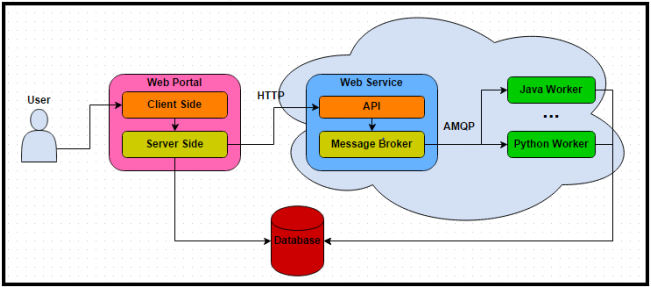
\includegraphics{architecture.png}
\end{figure}


\section{Web Portal}
\label{web_portal:library-web-portal}\label{web_portal::doc}\label{web_portal:web-portal}

\subsection{Introduction}
\label{web_portal:introduction}
\emph{Web Portal} is a part of our project which interacts with the user, like a
usual web-site. It is built with a Django Web Framework, Bootstrap Framework
and uses JavaScript, CodeMirror and prism.js library. It consists of several
modules: main, users, courses, errors.


\subsection{Deployment}
\label{web_portal:deployment}
This part of the documentation covers the deployment of \emph{Web Portal} on local
system. The first step to using any software package is getting it properly
installed.


\subsubsection{Get the Code}
\label{web_portal:get-the-code}
\emph{Web Portal} is actively developed on GitHub, where the code is
\href{https://github.com/azastupailo/Code-Project}{always available}.

You can either clone the public repository:

\begin{Verbatim}[commandchars=\\\{\}]
\PYGZdl{} git clone git://github.com/azastupailo/Code\PYGZhy{}Project.git
\end{Verbatim}


\subsubsection{Pip \& Virtualenv}
\label{web_portal:pip-virtualenv}
\code{pip} is a package management system used to install and manage software
packages written in Python.

Please install \code{pip} by following
\href{https://pip.pypa.io/en/latest/installing.html}{this link}.

\begin{notice}{warning}{Warning:}
Please don't proceed to the next steps before installing \code{pip}.
\end{notice}

\code{virtualenv} is a tool to create isolated Python environments. It creates
an environment that has its own installation directories, that doesn't share
libraries with other virtualenv environments (and optionally doesn't access
the globally installed libraries either).
You can install \code{python-virtualenv} and use for a project or you can use
your regular Python environment in the system. to install \code{virtualenv}
please follow \href{https://virtualenv.pypa.io/en/latest/installation.html}{this link}.

So, if you have installed \code{virtualenv}, first you need to create and
activate it:

\begin{Verbatim}[commandchars=\\\{\}]
\PYGZdl{} cd \PYGZlt{}code\PYGZhy{}project\PYGZhy{}dir\PYGZgt{}
\PYGZdl{} virtualenv venv
\PYGZdl{} source venv/bin/activate
\end{Verbatim}

To deactivate \code{virtualenv} later just simply type:

\begin{Verbatim}[commandchars=\\\{\}]
\PYGZdl{} deactivate
\end{Verbatim}

Now we can install all the dependecies for \emph{Web Portal}.

\begin{notice}{warning}{Warning:}
\emph{Web Portal} uses \code{PostgreSQL} database. Please make sure that it is installed in
your system.
\end{notice}

Installing python packages is simple, just run this in your terminal:

\begin{Verbatim}[commandchars=\\\{\}]
\PYGZdl{} pip install \PYGZhy{}r requirements.txt
\end{Verbatim}

Please specify database connection parameters in the \code{web\_portal/settings.py} file:

\begin{Verbatim}[commandchars=\\\{\}]
\PYG{n}{DATABASES} \PYG{o}{=} \PYG{p}{\PYGZob{}}
    \PYG{l+s}{\PYGZsq{}}\PYG{l+s}{default}\PYG{l+s}{\PYGZsq{}}\PYG{p}{:} \PYG{p}{\PYGZob{}}
        \PYG{l+s}{\PYGZsq{}}\PYG{l+s}{ENGINE}\PYG{l+s}{\PYGZsq{}}\PYG{p}{:} \PYG{l+s}{\PYGZsq{}}\PYG{l+s}{django.db.backends.postgresql\PYGZus{}psycopg2}\PYG{l+s}{\PYGZsq{}}\PYG{p}{,}
        \PYG{l+s}{\PYGZsq{}}\PYG{l+s}{NAME}\PYG{l+s}{\PYGZsq{}}\PYG{p}{:} \PYG{l+s}{\PYGZsq{}}\PYG{l+s}{database\PYGZhy{}name}\PYG{l+s}{\PYGZsq{}}\PYG{p}{,}
        \PYG{l+s}{\PYGZsq{}}\PYG{l+s}{USER}\PYG{l+s}{\PYGZsq{}}\PYG{p}{:} \PYG{l+s}{\PYGZsq{}}\PYG{l+s}{user\PYGZhy{}name}\PYG{l+s}{\PYGZsq{}}\PYG{p}{,}
        \PYG{l+s}{\PYGZsq{}}\PYG{l+s}{PASSWORD}\PYG{l+s}{\PYGZsq{}}\PYG{p}{:} \PYG{l+s}{\PYGZsq{}}\PYG{l+s}{password}\PYG{l+s}{\PYGZsq{}}\PYG{p}{,}
        \PYG{l+s}{\PYGZsq{}}\PYG{l+s}{HOST}\PYG{l+s}{\PYGZsq{}}\PYG{p}{:} \PYG{l+s}{\PYGZsq{}}\PYG{l+s}{host}\PYG{l+s}{\PYGZsq{}}\PYG{p}{,}
        \PYG{l+s}{\PYGZsq{}}\PYG{l+s}{PORT}\PYG{l+s}{\PYGZsq{}}\PYG{p}{:} \PYG{l+s}{\PYGZsq{}}\PYG{l+s}{port}\PYG{l+s}{\PYGZsq{}}\PYG{p}{,}
    \PYG{p}{\PYGZcb{}}
\PYG{p}{\PYGZcb{}}
\end{Verbatim}

And email parameters used for sending activation link to the users at \emph{Web Portal}:

\begin{Verbatim}[commandchars=\\\{\}]
\PYG{n}{DEFAULT\PYGZus{}EMAIL} \PYG{o}{=} \PYG{l+s}{\PYGZsq{}}\PYG{l+s}{my.email@gmail.com}\PYG{l+s}{\PYGZsq{}}
\PYG{n}{EMAIL\PYGZus{}HOST} \PYG{o}{=} \PYG{l+s}{\PYGZsq{}}\PYG{l+s}{smtp.gmail.com}\PYG{l+s}{\PYGZsq{}}
\PYG{n}{EMAIL\PYGZus{}PORT} \PYG{o}{=} \PYG{l+m+mi}{587}
\PYG{n}{EMAIL\PYGZus{}HOST\PYGZus{}USER} \PYG{o}{=} \PYG{l+s}{\PYGZsq{}}\PYG{l+s}{my.email}\PYG{l+s}{\PYGZsq{}}
\PYG{n}{EMAIL\PYGZus{}HOST\PYGZus{}PASSWORD} \PYG{o}{=} \PYG{l+s}{\PYGZsq{}}\PYG{l+s}{password}\PYG{l+s}{\PYGZsq{}}
\PYG{n}{EMAIL\PYGZus{}USE\PYGZus{}TLS} \PYG{o}{=} \PYG{n+nb+bp}{True}
\end{Verbatim}

Now let's synchronize the database now:

\begin{Verbatim}[commandchars=\\\{\}]
\PYGZdl{} python manage.py syncdb
\end{Verbatim}

And simply run the \emph{Web Portal}:

\begin{Verbatim}[commandchars=\\\{\}]
\PYGZdl{} python manage.py runserver
\end{Verbatim}


\subsection{Developer Interface}
\label{web_portal:developer-interface}
This part of the documentation covers all the interfaces of \emph{Web Portal}.
For parts where \emph{Web Portal} depends on external libraries, we document the most
important right here and provide links to the canonical documentation.

As we have already mentioned, \emph{Web Portal} consists of several modules:
main, users, courses and errors.


\subsubsection{main module}
\label{web_portal:main-module}
This module is responsible for following views:

\begin{Verbatim}[commandchars=\\\{\}]
http://your.domain.com/
http://your.domain.com/index
http://your.domain.com/coming
http://your.domain.com/our\PYGZhy{}team
\end{Verbatim}
\index{index() (in module core.main.views)}

\begin{fulllineitems}
\phantomsection\label{web_portal:core.main.views.index}\pysiglinewithargsret{\code{core.main.views.}\bfcode{index}}{\emph{request}}{}
Main page view. Generates index.html template.
\begin{quote}\begin{description}
\item[{Param}] \leavevmode
\emph{Request} object

\item[{Returns}] \leavevmode
\emph{HTTPResponse} object

\end{description}\end{quote}

\end{fulllineitems}

\index{coming() (in module core.main.views)}

\begin{fulllineitems}
\phantomsection\label{web_portal:core.main.views.coming}\pysiglinewithargsret{\code{core.main.views.}\bfcode{coming}}{\emph{request}}{}
Coming soon view. Generates coming.html template.
\begin{quote}\begin{description}
\item[{Param}] \leavevmode
\emph{Request} object

\item[{Returns}] \leavevmode
\emph{HTTPResponse} object

\end{description}\end{quote}

\end{fulllineitems}

\index{our\_team() (in module core.main.views)}

\begin{fulllineitems}
\phantomsection\label{web_portal:core.main.views.our_team}\pysiglinewithargsret{\code{core.main.views.}\bfcode{our\_team}}{\emph{request}}{}
Team members view. Generates our\_team.html template.
\begin{quote}\begin{description}
\item[{Param}] \leavevmode
\emph{Request} object

\item[{Returns}] \leavevmode
\emph{HTTPResponse} object

\end{description}\end{quote}

\end{fulllineitems}



\subsubsection{users module}
\label{web_portal:users-module}
This module is responsible for following views:

\begin{Verbatim}[commandchars=\\\{\}]
http://your.domain.com/accounts/register/
http://your.domain.com/accounts/register/complete/
http://your.domain.com/accounts/login/
http://your.domain.com/accounts/logout/
http://your.domain.com/accounts/activate/\PYGZlt{}activation\PYGZus{}key\PYGZgt{}/
http://your.domain.com/accounts/activate/complete/
\end{Verbatim}
\index{UserProfile (class in core.users.models)}

\begin{fulllineitems}
\phantomsection\label{web_portal:core.users.models.UserProfile}\pysiglinewithargsret{\strong{class }\code{core.users.models.}\bfcode{UserProfile}}{\emph{*args}, \emph{**kwargs}}{}
Model for storing user's avatar
\begin{quote}\begin{description}
\item[{User}] \leavevmode
\code{User} object

\item[{Avatar}] \leavevmode
image uploaded by the \code{User}

\end{description}\end{quote}

\end{fulllineitems}

\index{CustomRegistrationView (class in core.users.views)}

\begin{fulllineitems}
\phantomsection\label{web_portal:core.users.views.CustomRegistrationView}\pysiglinewithargsret{\strong{class }\code{core.users.views.}\bfcode{CustomRegistrationView}}{\emph{**kwargs}}{}
Extended \code{django.registration.RegistrationView} object with
\emph{title}.

\end{fulllineitems}

\index{AppUserForm (class in core.users.forms)}

\begin{fulllineitems}
\phantomsection\label{web_portal:core.users.forms.AppUserForm}\pysiglinewithargsret{\strong{class }\code{core.users.forms.}\bfcode{AppUserForm}}{\emph{*args}, \emph{**kwargs}}{}
Extended \code{django.registration.RegistrationFormUniqueEmail} form
with user's first name and last name

\end{fulllineitems}



\subsubsection{courses module}
\label{web_portal:courses-module}
This module is responsible for following views:

\begin{Verbatim}[commandchars=\\\{\}]
http://your.domain.com/courses/
http://your.domain.com/courses/add/
http://your.domain.com/courses/\PYGZlt{}course\PYGZus{}id\PYGZgt{}/
http://your.domain.com/courses/\PYGZlt{}course\PYGZus{}id\PYGZgt{}/delete/
http://your.domain.com/courses/\PYGZlt{}course\PYGZus{}id\PYGZgt{}/attend/
http://your.domain.com/courses/\PYGZlt{}course\PYGZus{}id\PYGZgt{}/assignments/add/
http://your.domain.com/courses/\PYGZlt{}course\PYGZus{}id\PYGZgt{}/assignments/\PYGZlt{}assignment\PYGZus{}id\PYGZgt{}/
http://your.domain.com/courses/\PYGZlt{}course\PYGZus{}id\PYGZgt{}/assignments/\PYGZlt{}assignment\PYGZus{}id\PYGZgt{}/solutions/
http://your.domain.com/courses/\PYGZlt{}course\PYGZus{}id\PYGZgt{}/assignments/\PYGZlt{}assignment\PYGZus{}id\PYGZgt{}/solutions/\PYGZlt{}solution\PYGZus{}id\PYGZgt{}/
http://your.domain.com/courses/\PYGZlt{}course\PYGZus{}id\PYGZgt{}/attendee/\PYGZlt{}attendee\PYGZus{}id\PYGZgt{}/solutions/
\end{Verbatim}


\paragraph{api.py}
\label{web_portal:api-py}\index{get\_courses() (in module core.courses.api)}

\begin{fulllineitems}
\phantomsection\label{web_portal:core.courses.api.get_courses}\pysiglinewithargsret{\code{core.courses.api.}\bfcode{get\_courses}}{\emph{**kwargs}}{}
Gets a list of all courses by sending a GET request.
\begin{quote}\begin{description}
\item[{Parameters}] \leavevmode
\textbf{**kwargs} -- Optional arguments that \code{request} takes.

\item[{Returns}] \leavevmode
Json-encoded content of a response, if any.

\end{description}\end{quote}

\end{fulllineitems}

\index{get\_course() (in module core.courses.api)}

\begin{fulllineitems}
\phantomsection\label{web_portal:core.courses.api.get_course}\pysiglinewithargsret{\code{core.courses.api.}\bfcode{get\_course}}{\emph{course\_id}, \emph{**kwargs}}{}
Gets a course by id by sending a GET request.
\begin{quote}\begin{description}
\item[{Parameters}] \leavevmode\begin{itemize}
\item {} 
\textbf{course\_id} (\href{http://docs.python.org/library/functions.html\#int}{\emph{int}}) -- Id of the course

\item {} 
\textbf{**kwargs} -- Optional arguments that \code{request} takes.

\end{itemize}

\item[{Returns}] \leavevmode
Json-encoded content of a response, if any.

\end{description}\end{quote}

\end{fulllineitems}

\index{get\_assignments() (in module core.courses.api)}

\begin{fulllineitems}
\phantomsection\label{web_portal:core.courses.api.get_assignments}\pysiglinewithargsret{\code{core.courses.api.}\bfcode{get\_assignments}}{\emph{course\_id}, \emph{clipped\_body=True}, \emph{**kwargs}}{}
Gets a list of all assignments of the course by sending a GET request.
\begin{quote}\begin{description}
\item[{Parameters}] \leavevmode\begin{itemize}
\item {} 
\textbf{course\_id} (\href{http://docs.python.org/library/functions.html\#int}{\emph{int}}) -- Id of the course

\item {} 
\textbf{clipped\_body} -- Return a full response if set to True, otherwise     return only \emph{assignment} attribute of a response.

\item {} 
\textbf{**kwargs} -- Optional arguments that \code{request} takes.

\end{itemize}

\item[{Returns}] \leavevmode
Json-encoded content of a response, if any.

\end{description}\end{quote}

\end{fulllineitems}

\index{get\_assignment() (in module core.courses.api)}

\begin{fulllineitems}
\phantomsection\label{web_portal:core.courses.api.get_assignment}\pysiglinewithargsret{\code{core.courses.api.}\bfcode{get\_assignment}}{\emph{course\_id}, \emph{assignment\_id}, \emph{**kwargs}}{}
Gets an assignment of the course by id by sending a GET request.
\begin{quote}\begin{description}
\item[{Parameters}] \leavevmode\begin{itemize}
\item {} 
\textbf{course\_id} (\href{http://docs.python.org/library/functions.html\#int}{\emph{int}}) -- Id of the course

\item {} 
\textbf{assignment\_id} (\href{http://docs.python.org/library/functions.html\#int}{\emph{int}}) -- Id of the assignment

\item {} 
\textbf{**kwargs} -- Optional arguments that \code{request} takes.

\end{itemize}

\item[{Returns}] \leavevmode
Json-encoded content of a response, if any.

\end{description}\end{quote}

\end{fulllineitems}

\index{get\_solutions() (in module core.courses.api)}

\begin{fulllineitems}
\phantomsection\label{web_portal:core.courses.api.get_solutions}\pysiglinewithargsret{\code{core.courses.api.}\bfcode{get\_solutions}}{\emph{course\_id}, \emph{assignment\_id}, \emph{**kwargs}}{}
Gets a list of all solutions of an assignment in the course by sending a
GET request.
\begin{quote}\begin{description}
\item[{Parameters}] \leavevmode\begin{itemize}
\item {} 
\textbf{course\_id} (\href{http://docs.python.org/library/functions.html\#int}{\emph{int}}) -- Id of the course

\item {} 
\textbf{assignment\_id} (\href{http://docs.python.org/library/functions.html\#int}{\emph{int}}) -- Id of the assignment

\item {} 
\textbf{**kwargs} -- Optional arguments that \code{request} takes.

\end{itemize}

\item[{Returns}] \leavevmode
Json-encoded content of a response, if any.

\end{description}\end{quote}

\end{fulllineitems}

\index{get\_attendee\_solutions() (in module core.courses.api)}

\begin{fulllineitems}
\phantomsection\label{web_portal:core.courses.api.get_attendee_solutions}\pysiglinewithargsret{\code{core.courses.api.}\bfcode{get\_attendee\_solutions}}{\emph{course\_id}, \emph{attendee\_id}, \emph{**kwargs}}{}
Gets a list of all solutions of an attendee in the course by sending a
GET request.
\begin{quote}\begin{description}
\item[{Parameters}] \leavevmode\begin{itemize}
\item {} 
\textbf{course\_id} (\href{http://docs.python.org/library/functions.html\#int}{\emph{int}}) -- Id of the course

\item {} 
\textbf{attendee\_id} (\href{http://docs.python.org/library/functions.html\#int}{\emph{int}}) -- Id of the attendee of the course

\item {} 
\textbf{**kwargs} -- Optional arguments that \code{request} takes.

\end{itemize}

\item[{Returns}] \leavevmode
Json-encoded content of a response, if any.

\end{description}\end{quote}

\end{fulllineitems}

\index{get\_user\_avatar\_url() (in module core.courses.api)}

\begin{fulllineitems}
\phantomsection\label{web_portal:core.courses.api.get_user_avatar_url}\pysiglinewithargsret{\code{core.courses.api.}\bfcode{get\_user\_avatar\_url}}{\emph{user\_id}}{}
Gets an url of the avatar of the user.
\begin{quote}\begin{description}
\item[{Parameters}] \leavevmode
\textbf{user\_id} (\href{http://docs.python.org/library/functions.html\#int}{\emph{int}}) -- Id of the user

\item[{Returns}] \leavevmode
Url to user's avatar

\end{description}\end{quote}

\end{fulllineitems}

\index{create\_course() (in module core.courses.api)}

\begin{fulllineitems}
\phantomsection\label{web_portal:core.courses.api.create_course}\pysiglinewithargsret{\code{core.courses.api.}\bfcode{create\_course}}{\emph{json\_data}, \emph{**kwargs}}{}
Creates a new course by sending a POST request.
\begin{quote}\begin{description}
\item[{Parameters}] \leavevmode\begin{itemize}
\item {} 
\textbf{json\_data} (\href{http://docs.python.org/library/stdtypes.html\#dict}{\emph{dict}}) -- Course json representation

\item {} 
\textbf{**kwargs} -- Optional arguments that \code{request} takes.

\end{itemize}

\item[{Returns}] \leavevmode
Url of the created course

\end{description}\end{quote}

\end{fulllineitems}

\index{create\_assignment() (in module core.courses.api)}

\begin{fulllineitems}
\phantomsection\label{web_portal:core.courses.api.create_assignment}\pysiglinewithargsret{\code{core.courses.api.}\bfcode{create\_assignment}}{\emph{course\_id}, \emph{json\_data}, \emph{**kwargs}}{}
Creates a new assignment by sending a POST request.
\begin{quote}\begin{description}
\item[{Parameters}] \leavevmode\begin{itemize}
\item {} 
\textbf{course\_id} (\href{http://docs.python.org/library/functions.html\#int}{\emph{int}}) -- Id of the course to create new assignment in

\item {} 
\textbf{json\_data} (\href{http://docs.python.org/library/stdtypes.html\#dict}{\emph{dict}}) -- Assignment json representation

\item {} 
\textbf{**kwargs} -- Optional arguments that \code{request} takes.

\end{itemize}

\item[{Returns}] \leavevmode
Url of the created assignment

\end{description}\end{quote}

\end{fulllineitems}

\index{create\_solution() (in module core.courses.api)}

\begin{fulllineitems}
\phantomsection\label{web_portal:core.courses.api.create_solution}\pysiglinewithargsret{\code{core.courses.api.}\bfcode{create\_solution}}{\emph{course\_id}, \emph{assignment\_id}, \emph{json\_data}, \emph{**kwargs}}{}
Creates a new solution by sending a POST request.
\begin{quote}\begin{description}
\item[{Parameters}] \leavevmode\begin{itemize}
\item {} 
\textbf{course\_id} (\href{http://docs.python.org/library/functions.html\#int}{\emph{int}}) -- Id of the course to create new solution in

\item {} 
\textbf{assignment\_id} (\href{http://docs.python.org/library/functions.html\#int}{\emph{int}}) -- Id of the assignment to create new solution in

\item {} 
\textbf{json\_data} (\href{http://docs.python.org/library/stdtypes.html\#dict}{\emph{dict}}) -- Solution json representation

\item {} 
\textbf{**kwargs} -- Optional arguments that \code{request} takes.

\end{itemize}

\item[{Returns}] \leavevmode
Url of the created solution

\end{description}\end{quote}

\end{fulllineitems}

\index{attend\_course() (in module core.courses.api)}

\begin{fulllineitems}
\phantomsection\label{web_portal:core.courses.api.attend_course}\pysiglinewithargsret{\code{core.courses.api.}\bfcode{attend\_course}}{\emph{course\_id}, \emph{**kwargs}}{}
Adds a user to the course by sending a POST request..
\begin{quote}\begin{description}
\item[{Parameters}] \leavevmode\begin{itemize}
\item {} 
\textbf{course\_id} (\href{http://docs.python.org/library/functions.html\#int}{\emph{int}}) -- Id of the course to create new solution in

\item {} 
\textbf{**kwargs} -- Optional arguments that \code{request} takes.

\end{itemize}

\item[{Returns}] \leavevmode
Url of the added attendee

\end{description}\end{quote}

\end{fulllineitems}

\index{delete\_course() (in module core.courses.api)}

\begin{fulllineitems}
\phantomsection\label{web_portal:core.courses.api.delete_course}\pysiglinewithargsret{\code{core.courses.api.}\bfcode{delete\_course}}{\emph{course\_id}, \emph{**kwargs}}{}
Deletes a course by sending a DELETE request.
\begin{quote}\begin{description}
\item[{Parameters}] \leavevmode\begin{itemize}
\item {} 
\textbf{course\_id} (\href{http://docs.python.org/library/functions.html\#int}{\emph{int}}) -- Id of the course to create new solution in

\item {} 
\textbf{**kwargs} -- Optional arguments that \code{request} takes.

\end{itemize}

\item[{Returns}] \leavevmode
Json-encoded content of a response, if any.

\end{description}\end{quote}

\end{fulllineitems}



\paragraph{forms.py}
\label{web_portal:forms-py}\index{SiteForm (class in core.courses.forms)}

\begin{fulllineitems}
\phantomsection\label{web_portal:core.courses.forms.SiteForm}\pysiglinewithargsret{\strong{class }\code{core.courses.forms.}\bfcode{SiteForm}}{\emph{*args}, \emph{**kwargs}}{}
Extended \code{Form} object. Removes `default :' after labels on the
form.

\end{fulllineitems}

\index{CourseForm (class in core.courses.forms)}

\begin{fulllineitems}
\phantomsection\label{web_portal:core.courses.forms.CourseForm}\pysiglinewithargsret{\strong{class }\code{core.courses.forms.}\bfcode{CourseForm}}{\emph{*args}, \emph{**kwargs}}{}
Extended \code{SiteForm} with \emph{name} and \emph{description} fields.

\end{fulllineitems}

\index{AssignmentForm (class in core.courses.forms)}

\begin{fulllineitems}
\phantomsection\label{web_portal:core.courses.forms.AssignmentForm}\pysiglinewithargsret{\strong{class }\code{core.courses.forms.}\bfcode{AssignmentForm}}{\emph{*args}, \emph{**kwargs}}{}
Extended \code{SiteForm} with \emph{name},{}`description{}`, \emph{language},
\emph{template\_code} and \emph{verification\_code} fields.

\end{fulllineitems}

\index{SolutionForm (class in core.courses.forms)}

\begin{fulllineitems}
\phantomsection\label{web_portal:core.courses.forms.SolutionForm}\pysiglinewithargsret{\strong{class }\code{core.courses.forms.}\bfcode{SolutionForm}}{\emph{*args}, \emph{**kwargs}}{}
Extended \code{SiteForm} with \emph{code} field.

\end{fulllineitems}



\paragraph{views.py}
\label{web_portal:views-py}\index{course\_list() (in module core.courses.views)}

\begin{fulllineitems}
\phantomsection\label{web_portal:core.courses.views.course_list}\pysiglinewithargsret{\code{core.courses.views.}\bfcode{course\_list}}{\emph{request}, \emph{*args}, \emph{**kwargs}}{}
Course list view. Gets a list of courses, paginates and generates
\emph{courses/course\_list.html} template as a response.
\begin{quote}\begin{description}
\item[{Parameters}] \leavevmode
\textbf{request} -- \code{Request} object

\item[{Returns}] \leavevmode
\code{HttpResponse} object

\end{description}\end{quote}

\end{fulllineitems}

\index{course\_page() (in module core.courses.views)}

\begin{fulllineitems}
\phantomsection\label{web_portal:core.courses.views.course_page}\pysiglinewithargsret{\code{core.courses.views.}\bfcode{course\_page}}{\emph{request}, \emph{*args}, \emph{**kwargs}}{}
Course page view. Gets a course and generates \emph{courses/course\_page.html}
template as a response.
\begin{quote}\begin{description}
\item[{Parameters}] \leavevmode\begin{itemize}
\item {} 
\textbf{request} -- \code{Request} object

\item {} 
\textbf{course\_id} (\href{http://docs.python.org/library/functions.html\#int}{\emph{int}}) -- Id of the requested course

\end{itemize}

\item[{Returns}] \leavevmode
\code{HttpResponse} object

\end{description}\end{quote}

\end{fulllineitems}

\index{assignment\_page() (in module core.courses.views)}

\begin{fulllineitems}
\phantomsection\label{web_portal:core.courses.views.assignment_page}\pysiglinewithargsret{\code{core.courses.views.}\bfcode{assignment\_page}}{\emph{request}, \emph{*args}, \emph{**kwargs}}{}
Assignment page view. Gets a course and generates \emph{courses/assignment\_page.html}
template as a response.
\begin{quote}\begin{description}
\item[{Parameters}] \leavevmode\begin{itemize}
\item {} 
\textbf{request} -- \code{Request} object

\item {} 
\textbf{course\_id} (\href{http://docs.python.org/library/functions.html\#int}{\emph{int}}) -- Id of the course to which requested assignment belongs

\item {} 
\textbf{assignment\_id} (\href{http://docs.python.org/library/functions.html\#int}{\emph{int}}) -- Id of the requested assignment

\end{itemize}

\item[{Returns}] \leavevmode
\code{HttpResponse} object

\end{description}\end{quote}

\end{fulllineitems}

\index{solution\_page() (in module core.courses.views)}

\begin{fulllineitems}
\phantomsection\label{web_portal:core.courses.views.solution_page}\pysiglinewithargsret{\code{core.courses.views.}\bfcode{solution\_page}}{\emph{request}, \emph{*args}, \emph{**kwargs}}{}
Solution page view. Gets a course and generates \emph{courses/solution\_page.html}
template as a response.
\begin{quote}\begin{description}
\item[{Parameters}] \leavevmode\begin{itemize}
\item {} 
\textbf{request} -- \code{Request} object

\item {} 
\textbf{course\_id} (\href{http://docs.python.org/library/functions.html\#int}{\emph{int}}) -- Id of the course to which requested solution belongs

\item {} 
\textbf{assignment\_id} (\href{http://docs.python.org/library/functions.html\#int}{\emph{int}}) -- Id of the assignment to which requested solution belongs

\item {} 
\textbf{solution\_id} (\href{http://docs.python.org/library/functions.html\#int}{\emph{int}}) -- Id of the requested solution

\end{itemize}

\item[{Returns}] \leavevmode
\code{HttpResponse} object

\end{description}\end{quote}

\end{fulllineitems}

\index{add\_course() (in module core.courses.views)}

\begin{fulllineitems}
\phantomsection\label{web_portal:core.courses.views.add_course}\pysiglinewithargsret{\code{core.courses.views.}\bfcode{add\_course}}{\emph{request}, \emph{*args}, \emph{**kwargs}}{}
Add course view. Gets a data from the form and requests an API create a
new course with this data.
\begin{quote}\begin{description}
\item[{Parameters}] \leavevmode
\textbf{request} -- \code{Request} object

\item[{Raises}] \leavevmode
\code{HttpResponseBadRequest}

\item[{Returns}] \leavevmode
\code{HttpResponse} object

\end{description}\end{quote}

\end{fulllineitems}

\index{add\_assignment() (in module core.courses.views)}

\begin{fulllineitems}
\phantomsection\label{web_portal:core.courses.views.add_assignment}\pysiglinewithargsret{\code{core.courses.views.}\bfcode{add\_assignment}}{\emph{request}, \emph{*args}, \emph{**kwargs}}{}
Add assignment view. Gets a data from the form and requests an API create a
new assignment with this data in a course.
\begin{quote}\begin{description}
\item[{Parameters}] \leavevmode\begin{itemize}
\item {} 
\textbf{request} -- \code{Request} object

\item {} 
\textbf{course\_id} (\href{http://docs.python.org/library/functions.html\#int}{\emph{int}}) -- Id of the course to create a new assignment in

\end{itemize}

\item[{Raises}] \leavevmode
\code{HttpResponseBadRequest}

\item[{Returns}] \leavevmode
\code{HttpResponse} object

\end{description}\end{quote}

\end{fulllineitems}

\index{add\_solution() (in module core.courses.views)}

\begin{fulllineitems}
\phantomsection\label{web_portal:core.courses.views.add_solution}\pysiglinewithargsret{\code{core.courses.views.}\bfcode{add\_solution}}{\emph{request}, \emph{*args}, \emph{**kwargs}}{}
Add solution view. Gets a data from the form and requests an API create a
new solution with this data in an assignment in the course.
\begin{quote}\begin{description}
\item[{Parameters}] \leavevmode\begin{itemize}
\item {} 
\textbf{request} -- \code{Request} object

\item {} 
\textbf{course\_id} (\href{http://docs.python.org/library/functions.html\#int}{\emph{int}}) -- Id of the course to create a new solution in

\item {} 
\textbf{assignment\_id} (\href{http://docs.python.org/library/functions.html\#int}{\emph{int}}) -- Id of the assignment to create a new solution in

\end{itemize}

\item[{Raises}] \leavevmode
\code{HttpResponseBadRequest}

\item[{Returns}] \leavevmode
\code{HttpResponse} object

\end{description}\end{quote}

\end{fulllineitems}

\index{attend\_course() (in module core.courses.views)}

\begin{fulllineitems}
\phantomsection\label{web_portal:core.courses.views.attend_course}\pysiglinewithargsret{\code{core.courses.views.}\bfcode{attend\_course}}{\emph{request}, \emph{*args}, \emph{**kwargs}}{}
Attend course view. Requests an API to add a user to the course.
\begin{quote}\begin{description}
\item[{Parameters}] \leavevmode\begin{itemize}
\item {} 
\textbf{request} -- \code{Request} object

\item {} 
\textbf{course\_id} (\href{http://docs.python.org/library/functions.html\#int}{\emph{int}}) -- Id of the course to add new user at

\end{itemize}

\item[{Raises}] \leavevmode
\code{HttpResponseBadRequest}

\item[{Returns}] \leavevmode
\code{HttpResponseRedirect} object

\end{description}\end{quote}

\end{fulllineitems}

\index{attendee\_solutions() (in module core.courses.views)}

\begin{fulllineitems}
\phantomsection\label{web_portal:core.courses.views.attendee_solutions}\pysiglinewithargsret{\code{core.courses.views.}\bfcode{attendee\_solutions}}{\emph{request}, \emph{*args}, \emph{**kwargs}}{}
Attendee solutions view. Gets a list of attendee solutions, and generates
\emph{courses/attendee\_solutions.html} template as a response.
\begin{quote}\begin{description}
\item[{Parameters}] \leavevmode\begin{itemize}
\item {} 
\textbf{request} -- \code{Request} object

\item {} 
\textbf{course\_id} (\href{http://docs.python.org/library/functions.html\#int}{\emph{int}}) -- Id of the course to add new user at

\item {} 
\textbf{attendee\_id} (\href{http://docs.python.org/library/functions.html\#int}{\emph{int}}) -- Id of the attendee to get solutions of

\end{itemize}

\item[{Returns}] \leavevmode
\code{HttpResponse} object

\end{description}\end{quote}

\end{fulllineitems}

\index{delete\_course() (in module core.courses.views)}

\begin{fulllineitems}
\phantomsection\label{web_portal:core.courses.views.delete_course}\pysiglinewithargsret{\code{core.courses.views.}\bfcode{delete\_course}}{\emph{request}, \emph{*args}, \emph{**kwargs}}{}
Delete course view. Requests an API to delete a course.
\begin{quote}\begin{description}
\item[{Parameters}] \leavevmode\begin{itemize}
\item {} 
\textbf{request} -- \code{Request} object

\item {} 
\textbf{course\_id} -- Id of the course to delete

\end{itemize}

\item[{Returns}] \leavevmode
\code{HttpResponseRedirect} object

\end{description}\end{quote}

\end{fulllineitems}



\paragraph{utils.py}
\label{web_portal:utils-py}\index{base\_request\_url() (in module core.courses.utils)}

\begin{fulllineitems}
\phantomsection\label{web_portal:core.courses.utils.base_request_url}\pysiglinewithargsret{\code{core.courses.utils.}\bfcode{base\_request\_url}}{\emph{path}}{}
Decorator for API that adds server address to the url beginning.
\begin{quote}\begin{description}
\item[{Parameters}] \leavevmode
\textbf{path} (\href{http://docs.python.org/library/functions.html\#str}{\emph{str}}) -- url

\end{description}\end{quote}

\end{fulllineitems}

\index{json\_object\_hook() (in module core.courses.utils)}

\begin{fulllineitems}
\phantomsection\label{web_portal:core.courses.utils.json_object_hook}\pysiglinewithargsret{\code{core.courses.utils.}\bfcode{json\_object\_hook}}{\emph{response}}{}
Convert JSON representation of response to object one.
\begin{quote}\begin{description}
\item[{Parameters}] \leavevmode
\textbf{response} -- \code{HTTPResponse} object

\item[{Returns}] \leavevmode
\code{JSONResponse} object

\end{description}\end{quote}

\end{fulllineitems}

\index{get\_page\_from\_request() (in module core.courses.utils)}

\begin{fulllineitems}
\phantomsection\label{web_portal:core.courses.utils.get_page_from_request}\pysiglinewithargsret{\code{core.courses.utils.}\bfcode{get\_page\_from\_request}}{\emph{request}, \emph{key='page'}}{}
Get current page number from the request
\begin{quote}\begin{description}
\item[{Parameters}] \leavevmode\begin{itemize}
\item {} 
\textbf{request} -- \code{Request} object

\item {} 
\textbf{key} (\href{http://docs.python.org/library/functions.html\#str}{\emph{str}}) -- Optional key to extract from the query string instead of page

\end{itemize}

\item[{Returns}] \leavevmode
Page number

\end{description}\end{quote}

\end{fulllineitems}

\index{user\_is\_attendee() (in module core.courses.utils)}

\begin{fulllineitems}
\phantomsection\label{web_portal:core.courses.utils.user_is_attendee}\pysiglinewithargsret{\code{core.courses.utils.}\bfcode{user\_is\_attendee}}{\emph{user}, \emph{attendees}}{}
Check whether current user is in the attendees list.
\begin{quote}\begin{description}
\item[{Parameters}] \leavevmode\begin{itemize}
\item {} 
\textbf{user} -- \code{User} object

\item {} 
\textbf{attendees} -- a list of \code{User} objects, who are attendees of the course

\end{itemize}

\item[{Returns}] \leavevmode
\emph{True} if a user is attendee, \emph{False} otherwise

\end{description}\end{quote}

\end{fulllineitems}

\index{user\_is\_organizer() (in module core.courses.utils)}

\begin{fulllineitems}
\phantomsection\label{web_portal:core.courses.utils.user_is_organizer}\pysiglinewithargsret{\code{core.courses.utils.}\bfcode{user\_is\_organizer}}{\emph{user}, \emph{organizer}}{}
Check whether current user is organizer of the course.
\begin{quote}\begin{description}
\item[{Parameters}] \leavevmode\begin{itemize}
\item {} 
\textbf{user} -- \code{User} object

\item {} 
\textbf{organizer} -- \code{User} object representing organizer of the course

\end{itemize}

\item[{Returns}] \leavevmode
\emph{True} if a user is organizer, \emph{False} otherwise

\end{description}\end{quote}

\end{fulllineitems}

\index{process\_request() (in module core.courses.utils)}

\begin{fulllineitems}
\phantomsection\label{web_portal:core.courses.utils.process_request}\pysiglinewithargsret{\code{core.courses.utils.}\bfcode{process\_request}}{\emph{method}, \emph{url}, \emph{data=None}, \emph{return\_only\_body=True}, \emph{**kwargs}}{}
Process request by send it, check its status and return response.
\begin{quote}\begin{description}
\item[{Parameters}] \leavevmode\begin{itemize}
\item {} 
\textbf{method} -- Method of the \code{request}.

\item {} 
\textbf{url} -- URL for the new \code{Request} object.

\item {} 
\textbf{data} -- (optional) Dictionary, bytes, or file-like object to send in the body of the POST \code{Request}.

\item {} 
\textbf{return\_only\_body} -- Return only message-body of the response as JSON-view object.

\item {} 
\textbf{**kwargs} -- Optional arguments that \code{request} takes.

\end{itemize}

\item[{Returns}] \leavevmode
\code{HTTPResponse} object if \emph{return\_only\_body} set to \emph{False},else \code{JSONResponse} object

\end{description}\end{quote}

\end{fulllineitems}

\index{send\_get\_request() (in module core.courses.utils)}

\begin{fulllineitems}
\phantomsection\label{web_portal:core.courses.utils.send_get_request}\pysiglinewithargsret{\code{core.courses.utils.}\bfcode{send\_get\_request}}{\emph{url}, \emph{*args}, \emph{**kwargs}}{}
Sends a GET request.
\begin{quote}\begin{description}
\item[{Parameters}] \leavevmode\begin{itemize}
\item {} 
\textbf{url} -- URL for the new \code{Request} object.

\item {} 
\textbf{headers} -- Headers used for the new \code{Request} object.

\item {} 
\textbf{**kwargs} -- Optional arguments that \code{request} takes.

\end{itemize}

\item[{Returns}] \leavevmode
\code{Response} object.

\end{description}\end{quote}

\end{fulllineitems}

\index{send\_post\_request() (in module core.courses.utils)}

\begin{fulllineitems}
\phantomsection\label{web_portal:core.courses.utils.send_post_request}\pysiglinewithargsret{\code{core.courses.utils.}\bfcode{send\_post\_request}}{\emph{url}, \emph{*args}, \emph{**kwargs}}{}
Sends a POST request.
\begin{quote}\begin{description}
\item[{Parameters}] \leavevmode\begin{itemize}
\item {} 
\textbf{url} -- URL for the new \code{Request} object.

\item {} 
\textbf{headers} -- Headers used for the new :class: \emph{Request} object.

\item {} 
\textbf{data} -- (optional) Dictionary, bytes, or file-like object to send in the body of the \code{Request}.

\item {} 
\textbf{**kwargs} -- Optional arguments that \code{request} takes.

\end{itemize}

\item[{Returns}] \leavevmode
\code{Response} object.

\end{description}\end{quote}

\end{fulllineitems}

\index{send\_delete\_request() (in module core.courses.utils)}

\begin{fulllineitems}
\phantomsection\label{web_portal:core.courses.utils.send_delete_request}\pysiglinewithargsret{\code{core.courses.utils.}\bfcode{send\_delete\_request}}{\emph{url}, \emph{*args}, \emph{**kwargs}}{}
Sends a DELETE request.
\begin{quote}\begin{description}
\item[{Parameters}] \leavevmode\begin{itemize}
\item {} 
\textbf{url} -- URL for the new \code{Request} object.

\item {} 
\textbf{**kwargs} -- Optional arguments that \code{request} takes.

\end{itemize}

\item[{Returns}] \leavevmode
\code{Response} object.

\end{description}\end{quote}

\end{fulllineitems}

\index{prepare\_headers() (in module core.courses.utils)}

\begin{fulllineitems}
\phantomsection\label{web_portal:core.courses.utils.prepare_headers}\pysiglinewithargsret{\code{core.courses.utils.}\bfcode{prepare\_headers}}{\emph{current\_headers}, \emph{obligatory\_headers}}{}
Adds \emph{obligatory\_headers} to \emph{current\_headers} if they are not already
included.
\begin{quote}\begin{description}
\item[{Parameters}] \leavevmode\begin{itemize}
\item {} 
\textbf{current\_headers} -- Dict of original headers

\item {} 
\textbf{obligatory\_headers} -- Dict of obligatory headers, which should be added

\end{itemize}

\item[{Returns}] \leavevmode
dictionary of headers

\end{description}\end{quote}

\end{fulllineitems}



\subsubsection{errors module}
\label{web_portal:errors-module}
This module is responsible for following custome errors views.


\paragraph{views.py}
\label{web_portal:id2}\index{bad\_request() (in module core.errors.views)}

\begin{fulllineitems}
\phantomsection\label{web_portal:core.errors.views.bad_request}\pysiglinewithargsret{\code{core.errors.views.}\bfcode{bad\_request}}{\emph{request}}{}
Bad request view. Generates \emph{errors/400.html} template.
\begin{quote}\begin{description}
\item[{Param}] \leavevmode
\code{Request} object

\item[{Returns}] \leavevmode
\code{HTTPResponse} object

\end{description}\end{quote}

\end{fulllineitems}

\index{permission\_denied() (in module core.errors.views)}

\begin{fulllineitems}
\phantomsection\label{web_portal:core.errors.views.permission_denied}\pysiglinewithargsret{\code{core.errors.views.}\bfcode{permission\_denied}}{\emph{request}}{}
Permission denied view. Generates \emph{errors/403.html} template.
\begin{quote}\begin{description}
\item[{Param}] \leavevmode
\code{Request} object

\item[{Returns}] \leavevmode
\code{HTTPResponse} object

\end{description}\end{quote}

\end{fulllineitems}

\index{page\_not\_found() (in module core.errors.views)}

\begin{fulllineitems}
\phantomsection\label{web_portal:core.errors.views.page_not_found}\pysiglinewithargsret{\code{core.errors.views.}\bfcode{page\_not\_found}}{\emph{request}}{}
Page not found view. Generates \emph{errors/404.html} template.
\begin{quote}\begin{description}
\item[{Param}] \leavevmode
\code{Request} object

\item[{Returns}] \leavevmode
\code{HTTPResponse} object

\end{description}\end{quote}

\end{fulllineitems}

\index{server\_error() (in module core.errors.views)}

\begin{fulllineitems}
\phantomsection\label{web_portal:core.errors.views.server_error}\pysiglinewithargsret{\code{core.errors.views.}\bfcode{server\_error}}{\emph{request}}{}
Internal server error view. Generates \emph{errors/500.html} template.
\begin{quote}\begin{description}
\item[{Param}] \leavevmode
\code{Request} object

\item[{Returns}] \leavevmode
\code{HTTPResponse} object

\end{description}\end{quote}

\end{fulllineitems}



\section{Support}
\label{support:support}\label{support::doc}
If you have questions or issues about \textbf{CODE} project, there are several options:


\subsection{File an Issue}
\label{support:file-an-issue}
If you notice some unexpected behaviour in \emph{Web Portal}, or want to see support
for a new feature,
\href{https://github.com/azastupailo/Code-Project/issues}{file an issue on GitHub}.


\subsection{E-mail}
\label{support:e-mail}
I'm more than happy to answer any personal or in-depth questions about
Requests. Feel free to email
\href{mailto:zastupailo@gmail.com}{zastupailo@gmail.com}.

I'm also available as \textbf{Oleksandr Zastupailo} on Facebook.



\renewcommand{\indexname}{Index}
\printindex
\end{document}
